\section{Model architecture}
\label{sec:model_architecture}

To solve the problem of error estimation, two different model architectures are devised. The first model architecture, FESDModelv1, is a deep convolutional neural network that takes the RGB, Depth, and Joint data as input. This model can be seen in figure \ref{fig:model_architecture_v1}. 


\begin{figure}[ht]
  \centering
  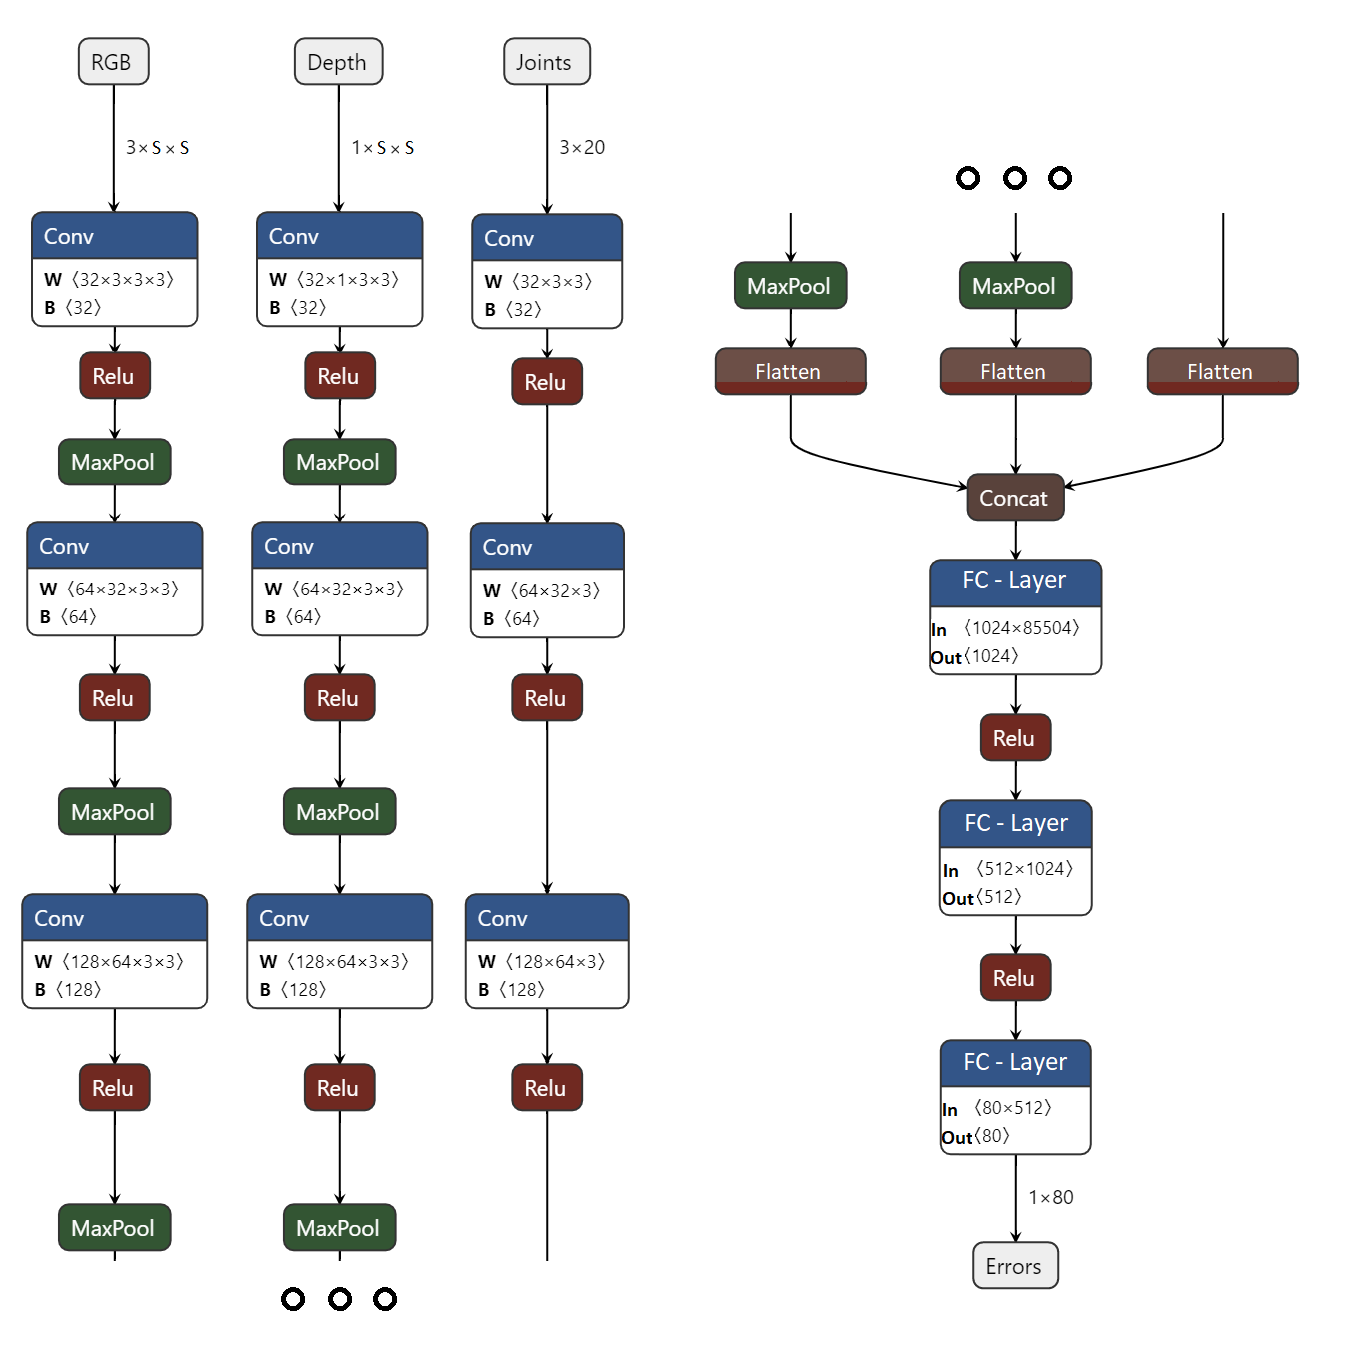
\includegraphics[width=.8\linewidth]{figures/Model/FESD.png}
  \caption[FESDModel architecture version 1]{Original FESDModel architecture with three different inputs; RGB, Depth and Joint data. After three convolutions the three streams are concatenated to be passed into three fully connected layers. In this example network, the model calculates the joint problem set, therefore the output is a 1D 80 tensor of multi-object, one for each joint, i.e. 20, multi-class, one for each error class, i.e. 4, values.}
  \label{fig:model_architecture_v1}
\end{figure}

The second model architecture, FESDModelv2, utilises transfer learning to extract the features of the input data using a pre-trained model. FESDModelv2 can be seen in figure \ref{fig:model_architecture_v2}. Both models are trained to predict the error labels for each joint. The error labels are the same as the error labels used in the data labelling. The error labels are explained in section \ref{sec:data_labeling}.

\begin{figure}[ht]
  \centering
  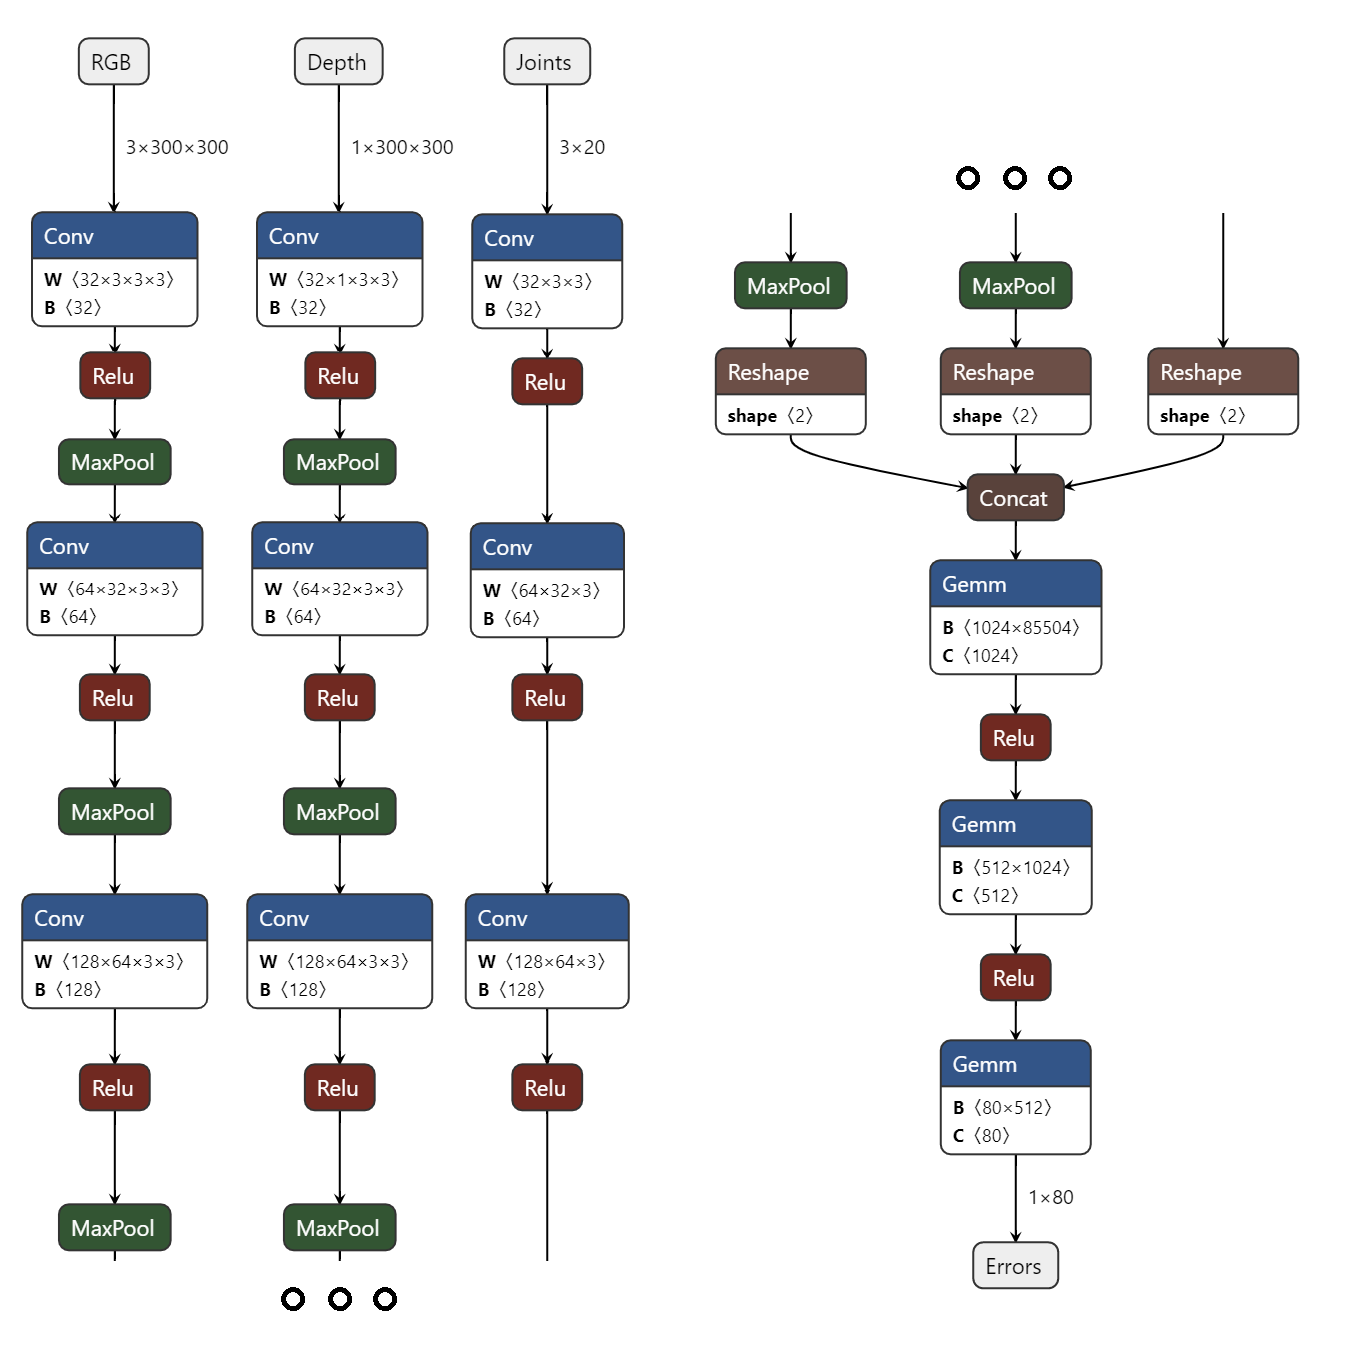
\includegraphics[width=.6\linewidth]{figures/Model/FESDv2.png}
  \caption[FESDModel architecture version 2]{FESDModelv2 architecture with transfer learning. The input is merged into a single RGB image and passed into a feature extractor. The feature extractor is a pre-trained EfficientNet v2 S. The output of the feature extractor is passed into two fully connected layers. In this example network, the model calculates the joint problem set, therefore the output is a 1D 80 tensor of multi-object, one for each joint, i.e. 20, multi-class, one for each error class, i.e. 4, values.}
  \label{fig:model_architecture_v2}
\end{figure}

While FESDModelv1 uses the data as it is stored in the dataset, FESDModelv2 merges the data into a single RGB image. This is done using the feature extractor, which is trained on RGB images. The data is merged by assigning each modality to a channel in an RGB image. The RGB image is transformed into greyscale and assigned to the red channel, the depth image is scaled to a value between 0 and 255 and assigned to the green channel, and the joint coordinates are assigned to the blue channel.

In total eight models were developed and trained. Four models were trained using FESDModelv1 and four models were trained using FESDModelv2. Each of the models for each version corresponds to one problem set, i.e. one model for each problem set is trained using FESDModelv1 and one model for each problem set is trained using FESDModelv2. The problem sets are explained in section \ref{sec:problem_set}.

Each of the four different models for each version of FESDModel has a different output vector. The full-body problem set has an output vector of size two. Each of the two values represents a boolean for "No Error" or "Error". To find if the result is an error or no error, the confidence rating and the most likely result is calculated using soft max(see section \ref{sec:fundamentals}). For every other problem set, the output vector is the number of Error classes, i.e. two, "No Error" and "Error", for the half-body and limb problem set, and four, "No Error", "Joint not Found", "Joint in a Wrong Position", "Joint at a Different Joint Position", for the joint problem set, times the number of objects. For example, the limb problem set has two error classes and six objects or areas, Head, Torso, Left and Right arm, and Left and Right Leg, therefore the output is a vector with 12 values. The output vector is split into the number of objects and the softmax is calculated for each object. 

To choose a network that is used by FESDModelv2 as a feature extractor, multiple different networks have been compared, which can be seen in figure \ref{fig:network_comparison}. One of the target applications of the model is to be used in a real time application so that error handling can be conducted. Consequently, a lightweight model which does not impact the performance much is preferred. Therefore, the models are compared by the number of floating-point operations (FLOPS) to their Accuracy on ImageNet-1K. Table \ref{tab:network_comparison} shows the top 5 models according to their accuracy and performance. 

\begin{figure}[ht]
  \centering
  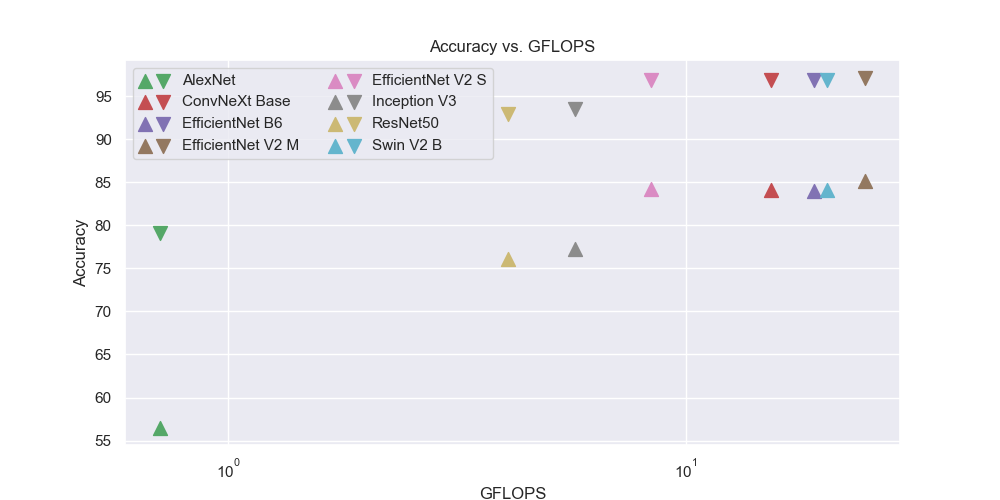
\includegraphics[width=\linewidth]{figures/network/networks.png}
  \caption[Network comparison]{The comparison of different networks by their GFLOPS and their Top-5 Accuracy. The models are sorted by their GFLOPS and their Top-5 Accuracy\footnote{Source: \url{https://pytorch.org/vision/main/models.html} on 08/05/2023}. The models are EfficientNet V2 S, ConvNeXt Base, EfficientNet B6, Swin V2 B, and EfficientNet V2 M. Additionally, AdamNet, ResNet-50 and Inception-v3 are added as a reference.}
  \label{fig:network_comparison}
\end{figure}

\begin{table}[ht]
  \caption[Top 5 models for Accuracy and Performance]{The top 5 models according to their accuracy and performance. The models are sorted by their GFLOPS and their Top-5 Accuracy\footnote{Source: \url{https://pytorch.org/vision/main/models.html} on 08/05/2023}. The models are EfficientNet V2 S, ConvNeXt Base, EfficientNet B6, Swin V2 B, and EfficientNet V2 M.}
  \label{tab:network_comparison}
  \centering
  \begin{tabular}{lrrrr}
    \hline
            Weight &  Acc@1 &  Acc@5 &   Params &  GFLOPS \\
    \hline
  EfficientNet V2 S & 84.228 & 96.878 & $2.15 \times 10^7$ &   8.370 \\
      ConvNeXt Base & 84.062 & 96.870 & $8.86 \times 10^7$ &  15.360 \\
    EfficientNet B6 & 84.008 & 96.916 & $4.30 \times 10^7$ &  19.070 \\
          Swin V2 B & 84.112 & 96.864 & $8.79 \times 10^7$ &  20.320 \\
  EfficientNet V2 M & 85.112 & 97.156 & $5.41 \times 10^7$ &  24.580 \\
  \hline
  \end{tabular}
\end{table}

EfficientNet v2 was chosen since it proved to be the most performant while being the most accurate of the networks that were analysed. In particular, the small variant with $2.15 \times 10^7$ Parameters and a Top-1 Accuracy of $84.228\%$. The model architecture can be seen in figure \ref{fig:model_architecture_v2}. The model is split into two parts. The first part is the feature extractor, which is the EfficientNet v2 S. The second part is the classifier, which is two fully connected Layers. The output of the classifier is a 1D 2, 4, 20, or 80 tensors of multi-object multi-class values depending on the problem set. Additionally, the input is merged into a single image so that EfficientNet v2 can be used to extract the features of all modalities.
